\chapter{Automatisierte UI Tests}
	\section{Einleitung} 
		\paragraph{} Automatisiertes UI-Testing bietet zahlreiche Vorteile in der Softwareentwicklung. Einige davon sind:
		
		\begin{itemize}
			\item Automatisierte Tests haben vergleichbare Ergebnisse und sind weniger anfällig für menschliche Fehler
			\item Höhere Testabdeckungsrate der Software
			\item Erhöhte Testabdeckung fördert debugging
			\item Erstellter Testcode kann wiederverwendet werden, wodurch das Testen leicht skalierbar wird
			\item Automatisierte Tests sind im Vergleich zu manuellen Tests viel schneller
			\item Sie sind Kosten- und Zeiteffizienter als manuelle Tests
		\end{itemize}		
		
		Der Global Quality Report zeigt, dass mehr als 60 \% der Unternehmen aufgrund der höheren Testabdeckung durch Testautomatisierung in der Lage sind, Fehler schneller zu erkennen. Darüber hinaus stellten 57 \% der Befragten fest, dass die Wiederverwendung von Testfällen durch den Einsatz von Automatisierung zunahm. Automatisiertes Testing gilt als de facto Standard in der Software Entwicklung \cite{capgemini2021microfocus}. 
		
		%Auch wenn automatisiertes Testing die nötigen manuellen Tests nicht vollständig ersetzen kann 
		
		Es äußerst wichtig, das richtige Gleichgewicht zwischen manuellen und automatisierten Tests zu finden. Jedes Projekt ist einzigartig, und es gilt, verschiedene Aspekte wie wirtschaftliche Machbarkeit, zeitliche Beschränkungen und die Art der durchzuführenden Tests zu berücksichtigen. Hier muss jedes Teams fundierte Entscheidungen treffen. Dieses Dokument dient als Entscheidungsgrundlage um ein Framework zu wählen, mit dem automatisierte UI Tests für Windows Qt-Anwendungen durchgeführt werden. Die Zielgruppe dieses Dokuments sind Softwareentwickler die mit dem C++ Qt Framework vertraut sind.
		
		\newpage
	\section{Anwendung}
		\paragraph{} Die Anwendung, die zum Vergleich der Frameworks verwendet wird, ist eine stark vereinfachte Version der Anlagensteuerungssoftware der Ambright GmbH.  
		
		\FloatBarrier
		\begin{figure}[t]		
			\centering
			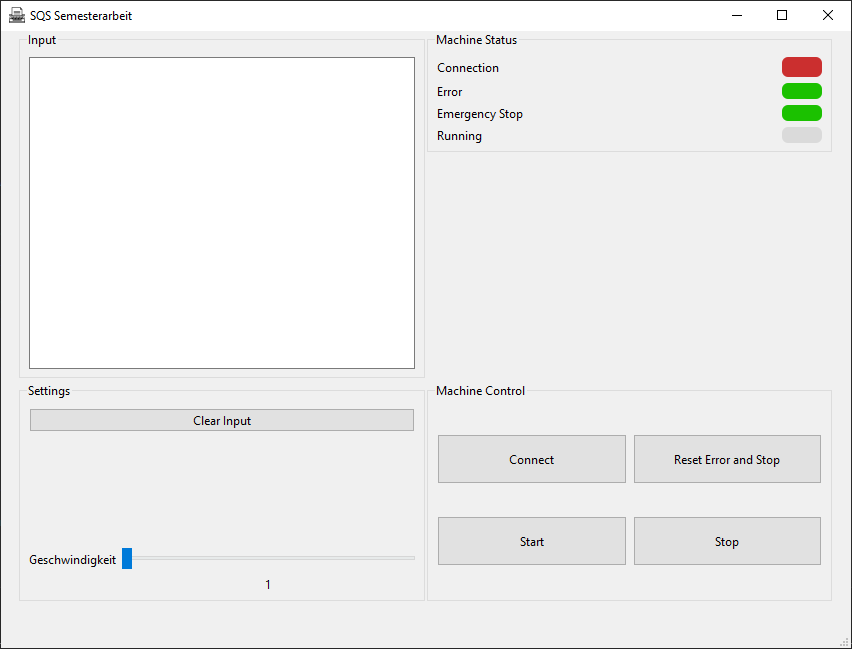
\includegraphics[width=\linewidth]{\figdir/Anwendung}
				
			\caption[Anwendung]
			{Anwendung an der die Tests Evaluiert werden}
			\label{FIG:Anwendung}
		\end{figure}
		\FloatBarrier
		
		\paragraph{} Die Anwendung (Abbildung \ref{FIG:Anwendung}) lässt sich in 4 Bereiche Unterteilen. Der erste Bereich, links oben, ist ein Text Feld. Dieses Text Feld kann mit User Input gefüllt werden. Der Input wird durch drücken des Start Buttons im vierten Bereich, rechts unten, evaluiert. Wenn der Input 'disconnect' oder 'error' beinhält werden entsprechende Methoden ausgeführt und der Status der Maschine verändert.  
		
		Im zweiten Bereich, rechts oben, sind 4 Statusanzeigen zu sehen. Die Statusanzeigen Signalisieren durch Farben den Status der Maschine. Wenn eine aktive Verbindung besteht ist die Anzeige der Connection grün, andernfalls rot. 
		Falls beim ausführen des Inputs aus dem ersten Bereich ein Fehler auftritt wird die Error Anzeige rot. Wenn kein Fehler auftritt ist sie grün eingefärbt. 
		Die Emergency Stop Anzeige zeigt an wenn der Nothalt Schalter gedrückt wurde mit roter Farbe. Falls der Nothalt Schalter nicht gedrückt wurde ist die Anzeige grün. 
		Die letzte Anzeige ist grün wenn gerade ein Script aus dem Inputfeld ausgeführt wird, und bleibt grün sofern keine Fehler auftreten oder Stop gedrückt wird.
		
		Im dritten Bereich, links unten, befinden sich Settings zur Maschine. Mit dem Button Clear Input werden alle Zeichen aus dem  Input Feld aus dem ersten Bereich entfernt. Durch den Slider kann die Geschwindigkeit innerhalb des Wertebereichs 1 bis 10 eingestellt werden. Der eingestellte Geschwindigkeitswert wird durch ein Label unter dem Slider angezeigt.
		
		Im letzten Bereich, rechts unten, befinden sich 4 Buttons. Der erste Button stellt eine Verbindung her. Der zweite Button setzt den Error Status zurück. Die letzten beiden Buttons sind zum Starten und Stoppen der Maschine.
		 
		 \newpage
	\section{Anforderungen}
		\paragraph{} Die Folgende Tabell (\ref{TAB:Anforderungstabelle}) gibt einen Überblick über die Anforderungen, welche an die UI Testing Frameworks gestellt werden. Anhand dieser Anforderungen werden die gewählten Frameworks verglichen und eine Entscheidung getroffen. Jede Anforderung ist mit einer ID versehen. Diese IDs werden im Dokument zur Referenzierung verwendet.
		%\begin{center}
					
			\begin{table}%[htdp]
				\caption{Anforderungstabelle}
				\label{TAB:Anforderungstabelle}
				\begin{tabularx}{\linewidth}{|s n g|}
				\hline
				ID & Anforderung & Metrik \\  
				\thickhline
				01 & Kosten & Kosten sollen so gering wie möglich sein \\ 
				\hline
				02 & Lizenz & Bestenfalls GPL oder vergleichbar \\
				\hline
				03 & Open Source & Source-Code öffentlich verfügbar  \\
				\hline
				04 & Integration in vorhandene Pipeline & Wie viel Zeit benötigt es die Tests in die Pipeline zu integrieren \\
				\hline
				05 & In Qt Editor ausführbar & Sind die Tests im Qt Editor ausführbar \\
				\hline 
				06 & Aufwand & Benötigte Zeit zum erstellen eines Tests \\
				\hline
				07 & Lesbarkeit & Kann der Testcode von Entwicklern gelesen werden \\  
				\hline
				08 & Änderbarkeit & Benötigte Zeit zum ändern eines Tests \\
				\hline				
				09 & Support / Community & Aktivität und Größe der Community (Stackoverflow, eigenes Forum, ...) \\
				\hline
				10 & Reife / Robustheit & Stabilität des Frameworks \\ 
				\hline
				11 & Updates & Update-Zyklus des Frameworks \\
				\hline				
				12 & Abdeckung der Qt Features & Mögliche Abdeckung der mit Qt erstellbaren Widgets  \\
				\hline 
				13 & Laufzeit & Wie viel Zeit beansprucht die Ausführung eines Tests \\
				\hline
				14 & Dokumentation & Umfang und Qualität der Dokumentation der Tests \\
				\hline
				15 & Auswertbarkeit der Ergebnisse & Lassen sich die Ergebnisse automatisiert auswerten \\
				\hline
			\end{tabularx}
		  \end{table}
		
		\FloatBarrier
	%	\end{center}
		
		\paragraph{}Anforderung [01] legt fest, dass die Kosten die für das UI Testing Framework anfallen sollen so gering wie möglich sein. Bestenfalls sollten keine Kosten anfallen. Dies ist direkt mit der Anforderung [02] verknüpft. Eine GNU General Public Lizenz oder vergleichbares wäre daher vorteilhaft. [03] Wenn der Source Code des UI Testing Frameworks frei verfügbar ist bestünde die Möglichkeit, Änderungen oder Ergänzungen am Framework vorzunehmen. Die Priorität von [03] ist als eher gering einzustufen. [04] Wenn das Framework nicht in die Verwendete Pipeline integriert werden kann, kann es nicht automatisiert verwendet werden und würde damit direkt ausgeschlossen werden. [05] Der beste Fall hierfür wäre die Möglichkeit die Tests im Qt Editor ausführen zu können. [06] Ebenso wichtig ist, wie viel Aufwand das schreiben oder Aufnehmen eines Tests ist, sowie die benötigte Zeit um mit dem Framework familär zu werden. [07] Dabei ist es ebenso Vorteilhaft wenn man den Testcode Lesen, nachvollziehen und verstehen kann. [08] Ebenso wird verglichen wie viel Aufwand eine Änderung eines Tests ist, wenn sich beispielsweise die Position eines Buttons verändert. [09] Zu untersuchen ist auch, wie groß die Community der Frameworks auf Seiten wie Stack Overflow, Github oder einem eigenem Forum ist. Mit Anforderung [10] wird sichergestellt dass Framework keine bekannten kritischen Bugs hat und bei ordnungsgemäßer Verwendung immer das selbe Ergebnis liefert. Dazu prüft [11] ob die Aussicht auf zukünftige Updates besteht. Ein weiteres Kriterium ist der Umfang des Frameworks. Mit [12] wird gemessen wie weit sich alle durch Qt bereit gestellten Widgets testen lassen und ob es die Möglichkeit gibt custom Widgets zu testen. Für den Konkreten Anwendungsfall sind nur Nutzerinteraktionen mit Tastatur und Maus zu erwarten. [13] Die Laufzeit der Tests ist ebenso ein bedeutendes Kriterium. Mit [14] wird der Umfang und die Qualität der Dokumentation der Frameworks verglichen. Zuletzt wird mit [15] getestet ob sich die Ergebnisse der Tests automatisiert auswerten lassen.

\chapter{Squish}
		
		\section{Squish}
		\paragraph{} Squish ist ein plattformübergreifendes UI- und regression test Tool, das eine Vielzahl von Anwendungen mit UIs testen kann. Unter anderem können Qt-, Java-, Web- und Mobile-Anwendungen getestet werden. Es wird von Froglogic entwickelt und gepflegt. Froglogic hat seinen Hauptsitz in Hamburg und bietet das Tool Squish seit 2003 an\cite{Squish}. Squish erlaubt es sowohl die UI Tests in der bereitgestellten IDE (Abbildung \ref{FIG:Squish}) aufzunehmen und durch die Aufnahme Code zu generieren, als auch den Testcode selbst zu schreiben. Der Testcode kann in JavaScript, Perl, Python, Ruby oder Tcl geschrieben, bzw. generiert werden.
		
		%\FloatBarrier
		\begin{figure}[t]		
			\centering
			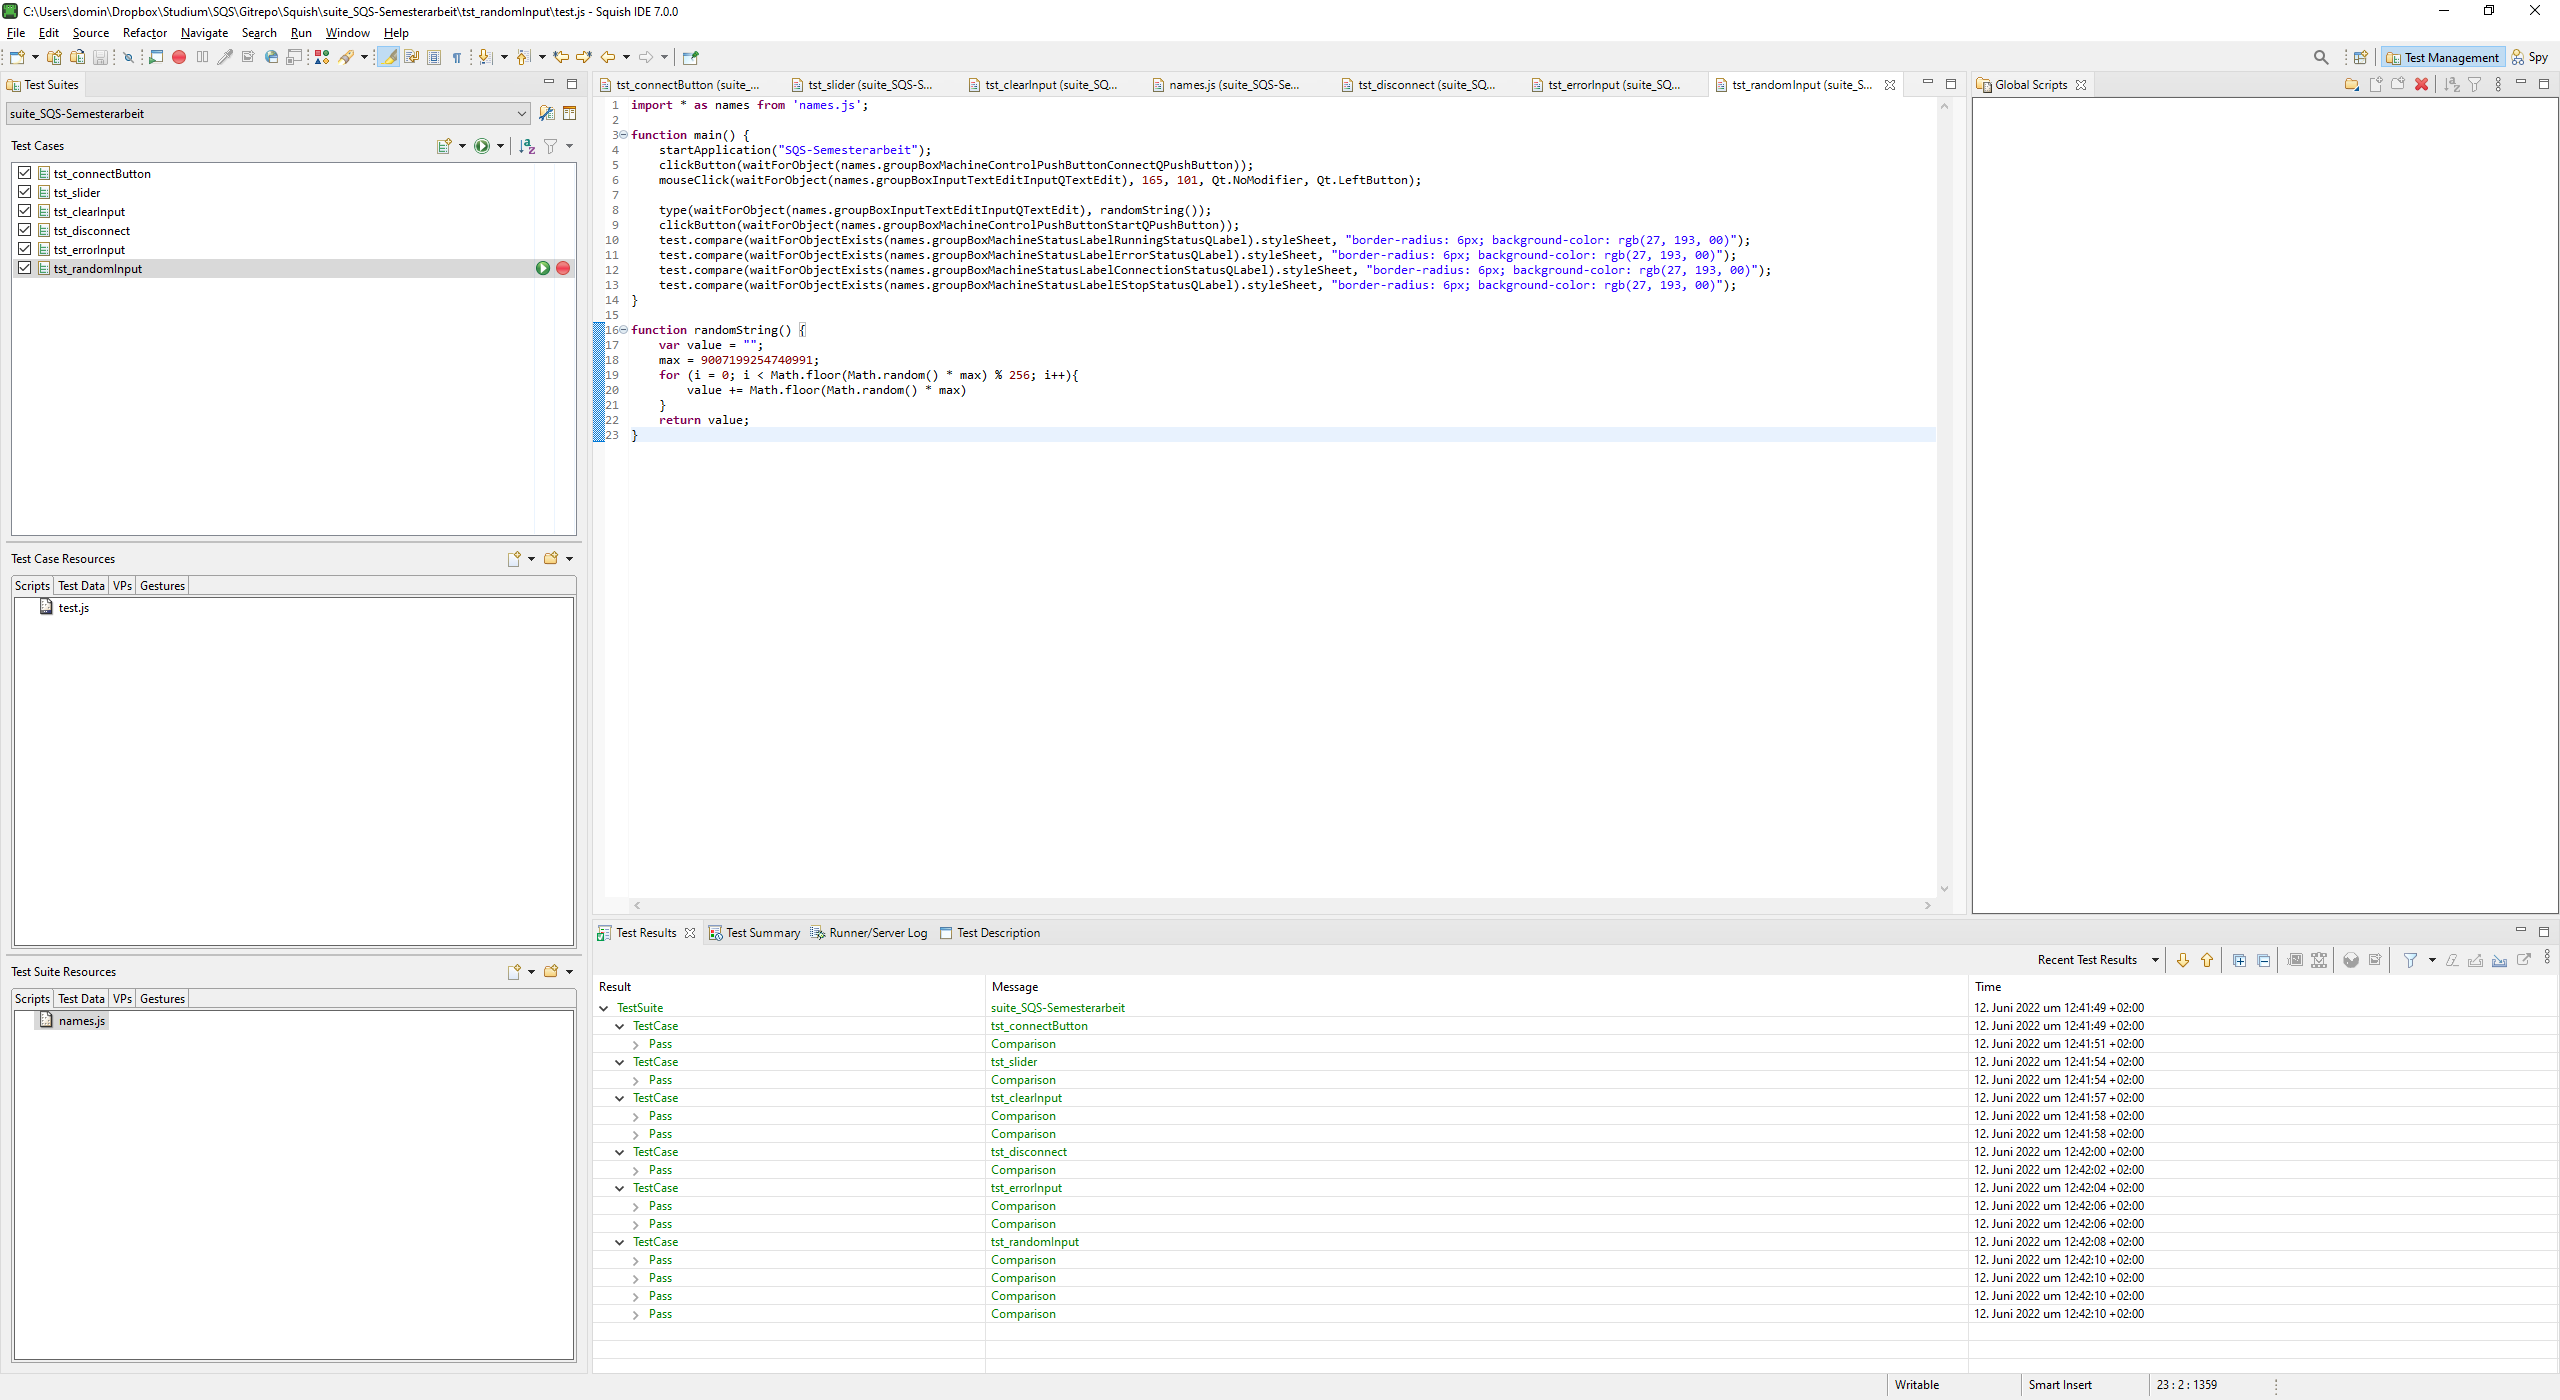
\includegraphics[width=\linewidth]{\figdir/Squish}
			
			\caption[Squish IDE]
			{Squish IDE in der die Tests erstellt werden}
			\label{FIG:Squish}
		\end{figure}
		\FloatBarrier
		
		\paragraph{} Als erster Schitt muss eine Test Suite angelegt werden. In der Test Suite wird das GUI toolkit, die Script Sprache der Tests sowie der Pfad zu der zu testenden Anwendung festgelegt. Das GUI toolkit legt fest für welche Art von Anwendung die Tests sind. In diesem Fall wurde Qt festgelegt. Zu einer Test Suite können beliebig viele Test Cases hinzugefügt werden. Die ausgewählte Test Suite sowie die Test Cases sind in der Squish IDE in der linken oberen Ecke angesiedelt (Ausgeschnitten in Abbildung \ref{FIG:testCasesSquish}). In der Mitte befindet sich der Script Editor, mit dem die erstellten Test Cases bearbeitet werden können. Unter dem Script Editor ist eine Anzeige bei der Zwischen den Testergebnissen, einer Zusammenfassung der Testergebnisse, den durch die Tests generierten Logs und der Beschreibung der Test Cases gewechselt werden kann. Um einen Test Case aufzunehmen muss der rote 'record' Button (Abbildung \ref{FIG:testCasesSquish})) gedrückt werden. Mit dem Start der Aufnahme wird sowohl die Anwendung als auch eine Control Bar (Abbildung \ref{FIG:controlBar})) zum steuern der Aufnahme geöffnet. Mit der Control Bar kann die Aufnahme beendet werden sowie Schritte zur Verifizierung als auch einfügen Nutzereingaben für die Anwendung in den Test eingefügt werden. Zur Verifizierung gibt es Verschiedene möglichkeiten. In dieser Arbeit wurde zur Verifizierung die Attribute einzelner UI Elemente abgeglichen. Andere Möglichkeiten wären beispielsweise abgleiche mit Screenshots oder Erkennung durch OCR.
		
		%\FloatBarrier
		\begin{figure}[t]		
			\centering
			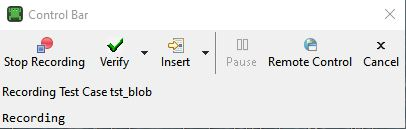
\includegraphics[width=\linewidth]{\figdir/controlBar}
			
			\caption[Squish IDE]
			{Control Bar mit der die Aufnahme eines Tests gesteuert wird}
			\label{FIG:controlBar}
		\end{figure}
		\FloatBarrier
		
		\section{Durchführung der Tests}
		\paragraph{} Um einen einzelnen Test oder die gesamte Test Suite zu starten gibt es verschiedene Möglichkeiten. Über die Squish IDE kann ein einzelner Test durch den Grünen Start Button neben dem Test gestartet werden (Abbildung \ref{FIG:testCasesSquish}). Die gesamte Test Suite wird über Run -> Run Test Suite ausgeführt. Um die Tests Automatisiert von der Command Line ausführen zu lassen benötigt es eine laufende Instanz eines squishservers. Squishserver gib es sowohl für Windows als auch Unix Systeme. Mit dem Command \textit{squishrunner --host <IP\_AddressOfSquishServer> --port 4322 --testsuite <PathToTestSuite>} wird die in dem Pfad hinterlegte Test Suite ausgeführt. Der squishserver wird über das Command \textit{squishrunner --host \%SQUISH\_SERVER\_HOST\% --port \%SQUISH\_SERVER\_PORT\% --testsuite \%TESTSUITE\% --reportgen xml2.1,\%REPORTPATH\%/report.xml} gestartet \cite{SquishCLI}. Die dadurch generierte report Datei kann automatisiert ausgewertet werden.
		
		\begin{figure}[t]		
			\centering
			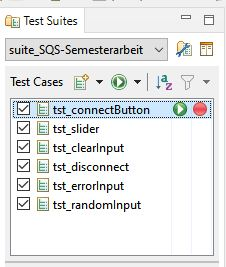
\includegraphics[width=\linewidth]{\figdir/testCasesSquish}
		
			\caption[Squish IDE]
			{Squish IDE, Ausschnitt der Test Suite und Test Cases}
			\label{FIG:testCasesSquish}
		\end{figure}
		\FloatBarrier
		
		\section{Tests}
		Mit dem Test tst\_connectButton wird überprüft ob durch drücken des Connect Buttons die Anzeige Connection grün wird. Dazu wird zuerst mit der Funktion startApplication() die Anwendung gestartet und danach mit der Funktion clickButton() der Connect Button angeklickt. Um zu überprüfen ob die Connected Anzeige grün ist wird die Funktion test.compare() aufgerufen.
		\begin{lstlisting}[language=JavaScript, caption=tst\_connectButton]
  function main() {
    startApplication("SQS-Semesterarbeit");
    clickButton(waitForObject(names.groupBoxMachineControlPushButtonConnectQPushButton));
    test.compare(waitForObjectExists(names.groupBoxMachineStatusLabelConnectionStatusQLabel).styleSheet, "border-radius: 6px; background-color: rgb(27, 193, 00)");
  }
		\end{lstlisting}
		
		Der zweite Test testet nach starten der Anwendung ob durch bewegen des Sliders das Label, dass die eingestellte Geschwindigkeit anzeigt wird korrekt aktualisiert wird. Der Slider wird durch die Funktion scrollTo() auf die Position 6 bewegt. Darauf folgend wird mit test.compare() verglichen ob das Label den richtigen Wert anzeigt.
		
		\begin{lstlisting}[language=JavaScript, caption=tst\_slider]
function main() {
  startApplication("SQS-Semesterarbeit");
  scrollTo(waitForObject(names.groupBoxSettingsHorizontalSliderSpeedQSlider), 6);
  test.compare(waitForObjectExists(names.groupBoxSettingsLabelSpeedValueQLabel).text, "6");
}

		\end{lstlisting}
		
		Durch den Test Case tst\_errorInput wird nach Anwendugsstart in das input Feld geklickt und dort der String 'error' über die Funktion type() als Keyboard Input eingegeben. Darauf folgend wird der Start Button gedrückt um die Maschine mit dem im Input stehenden Daten zu starten. Da dort 'error' steht wird erwartet, dass die Maschine in den Zustand Error wechselt. Um dies zu überprüfen wird das aussehen der Error Anzeige durch test.compare() abgeglichen.
		
		\begin{lstlisting}[language=JavaScript, caption=tst\_errorInput]
function main() {
  startApplication("SQS-Semesterarbeit");
  clickButton(waitForObject(names.groupBoxMachineControlPushButtonConnectQPushButton));
  mouseClick(waitForObject(names.groupBoxInputTextEditInputQTextEdit), 234, 156, Qt.NoModifier, Qt.LeftButton);
  type(waitForObject(names.groupBoxInputTextEditInputQTextEdit), "error");
  clickButton(waitForObject(names.groupBoxMachineControlPushButtonStartQPushButton));
  test.compare(waitForObjectExists(names.groupBoxMachineStatusLabelErrorStatusQLabel).styleSheet, "border-radius: 6px; background-color: rgb(203, 47, 47)");
  clickButton(waitForObject(names.groupBoxMachineControlPushButtonResetErrorAndEStopQPushButton));
  test.compare(waitForObjectExists(names.groupBoxMachineStatusLabelErrorStatusQLabel).styleSheet, "border-radius: 6px; background-color: rgb(27, 193, 00)");
}
\end{lstlisting}
		
\chapter{Qt Test}
		
		\section{Einführung Qt Test}
		\paragraph{} Qt ist ein cross-platform Framework zur Entwicklung von Desktop- , Embedded- und Mobile-Anwendungen. Qt ist keine eigenständige Programmiersprache, sondern ein in C++ geschriebenes Framework. Ein Präprozessor, der MOC (Meta-Object Compiler), wird verwendet, um die C++-Sprache um Funktionen wie Signals und Slots zu erweitern. Vor dem Kompilieren analysiert der MOC die in Qt-erweitertem C++ geschriebenen Quelldateien und erzeugt daraus standardkonforme C++-Quellendateien. Somit können das Framework selbst und die Anwendungen/Bibliotheken, die es verwenden, von jedem standardkonformen C++-Compiler kompiliert werden. Qt ist unter kommerziellen sowie open-source Lizenzen verfügbar. Das Framework befindet sich seit 1995 in Entwicklung und erhält seitdem regelmäßig Updates \cite{QtWiki}. Auf Stackoverflow gibt es derzeit 82.522 Fragen mit dem Tag Qt \cite{QtQuestions}. Zudem weißt das Qt Forum eine solide Aktivität auf. Daher ist von einer Mittelgroßen, aktiven Community auszugehen. Für dieses Projekt wird die Qt Version 5.15 verwendet.
				
		Qt Test ist ein Teil des Qt Frameworks. Es bietet Klassen für Unit-Tests von Qt-Anwendungen und -Bibliotheken. Alle öffentlichen Methoden befinden sich im QTest-Namensraum. Darüber hinaus bietet die Klasse QSignalSpy eine einfache Introspektion der Signale und Slots von Qt, und der QAbstractItemModelTester ermöglicht das nicht-destruktive Testen von Elementmodellen. Dadurch können auch UIs getestet werden. Es lassen sich Maus und Tastatur Eingaben durch ein von der Anwendung unabhängiges Eventsystem simulieren \cite{documentationQt}.
		
		Beispiel für einen Test:
		\begin{lstlisting}[language=C++, caption=Hello World Beispiel]
void TestGui::testGui()
{
  QLineEdit lineEdit;
	
  QTest::keyClicks(lineEdit, "hello world");
		
  QCOMPARE(lineEdit.text(), QString("hello world"));
}
		\end{lstlisting}
		\paragraph{} Die Methode TestGui::testGui() erstellt ein Eingabefeld. Durch die Methode QTest::keyClicks() wird das als Parameter übergebene QWdiget fokussiert und der als Parameter übergebene String als Tastatur Eingabe dem QWdiget übergeben. Mit dem Makro QCOMPARE() werden zwei Werte verglichen. Wenn die beiden übergebenen Werte den selben Inhalt haben wird das Programm fortgeführt. Sollte dies nicht der Fall ist wird der eine Fehlermeldung im Log ausgegeben und die Methode beendet. Für Mauseingaben gibt es mehrere Methoden. Unter anderem die Methoden QTest::mouseMove() und QTest::mouseClick(). QTest::mouseMove() bewegt den Mauszeiger auf die übergebene Position, ausgehend von dem Übergebenen QWdiget. QTest::mouseClick() führt einen Mausklick auf die übergebene Position für die übergebene Zeit aus.
		
		\newpage
		
		\section{Durchführung der Tests}
		\paragraph{} Die Tests werden durch folgende Zeilen in der main Methode aufgerufen:
		\begin{lstlisting}[language=C++, caption=main.cpp]
#ifdef QT_DEBUG
    TestSuite::executeTests();
#endif
		\end{lstlisting}
		Ob das QT\_DEBUG flag gesetzt ist hängt von den Parametern mit denen das Programm aufgerufen wird ab.
		
		Die Methode TestSuite::executeTests() führt alle registrierten Tests aus und meldet, ob sie erfolgreich waren oder nicht.
		\begin{lstlisting}[language=C++, caption=testsuite.cpp]
			
QList<QObject *> *TestSuite::m_suites = nullptr;

TestSuite::TestSuite()
{
  static bool init = true;
  if(init){
    m_suites = new QList<QObject *>;
    init = false;
  }
  m_suites->append(this);
}
		
void TestSuite::executeTests()
{
  if(m_suites == nullptr){
    qDebug() << "No tests available";
    return;
  }
	
  int failedTests = 0;
  QList<QObject*>::iterator it = m_suites->begin();
  for(;it != m_suites->end(); it++){
  	failedTests += QTest::qExec(*it);
  }
  qDebug() << "---------------------------------------";
  qDebug() << "Finished Testing";
  qDebug() << "Test Files: " << QString::number(m_suites->length());
  qDebug() << "Failed Tests: " << QString::number(failedTests);
  qDebug() << "---------------------------------------";
	
  if(failedTests != 0){
    exit(1);
  }
}
\end{lstlisting}
		Alle Testklassen registrieren sich durch eine statische instanz selbst in der QList<QObject *> m\_suites. Mit einem iterator wird durch die Liste m\_suites iteriert und jede Testklasse mit QTest::qExec() aufgerufen. QTest::qExec() führt alle Methoden in der Klasse auf die als private slots deklariert sind. Sollten darunter die Methoden initTestCase() oder init() deklariert sein, so werden diese vor jedem Test einzelnen Test, beziehungsweise vor allen Tests ausgeführt. Analog geschieht dies wenn die Methoden cleanupTestCase() oder cleanup() deklariert sind nach den Tests. QTest::qExec() gibt als Rückgabewert '0' falls keiner der Tests fehlgeschlagen ist, andernfalls die Anzahl an fehlgeschlagenen Methoden. Die Ergebnisse der Tests werden auf der Konsole ausgegeben und sollte ein oder mehrere Tests fehlgeschlagen sein wird das Programm beendet.
		
		\newpage
		
		\section{Tests}
		\paragraph{} Die Klasse QtGuiTest enthält 6 Tests, die den gleichen Ablauf haben wie die für Squish definierten Tests. Die Methode initTestCase(), die vor dem Durchlauf aller Tests aufgerufen wird, cleanupTestCase() welche nach dem Durchlauf aller Tests aufgerufen wird sowie zwei kleinen Methoden welche öfter in den Tests verwendet werden.
		
		\begin{lstlisting}[language=C++, caption=qtguitest.cpp]		
class QtGuiTest : public TestSuite
{
  Q_OBJECT
	
  friend class MainWindow;
	
  private Q_SLOTS:
  void initTestCase();
  void cleanupTestCase();
	
  void testConnectButton();
  void testSlider();
  void testClearInput();
  void testDisconnect();
  void testErrorInput();
  void testRandomInput();
	
  private:
  /**
  * @brief establishConnection: verifies that the machine is connected
  * using the GUI
  * @return true if there is a established connection, otherwise false
  */
  bool establishConnection();
	
  /**
  * @brief connectedAndRunning: Checks if the Machine is connected and
  * running
  * For Integrity it is also verified that there are no active errors
  * or that the emergency stop is activated
  * @return true if the machine is connected and running, otherwise
  * false
  */
  bool connectedAndRunning();
	
  private:
  QWidget *m_window;
};
		\end{lstlisting}
	
		Zudem ist die Klasse MainWindow als friend class markiert um auf die UI Elemente des MainWindows in den Tests zugreifen zu können. Ein Pointer auf eine Instanz von MainWindow wird in der Membervariable m\_window gespeichert.
		
		In QtGuiTest::initTestCase() wird die Membervariable m\_window initializiert und das Window angezeigt. Sollte das anzeigen des Windows fehlschlagen wird mit dem Makro QVERIFY2() ein Fehler ausgegeben.
		
		\begin{lstlisting}[language=C++, caption=qtguitest.cpp]	
void QtGuiTest::initTestCase()
{
  MainWindow *mainWindow = new MainWindow();
  m_window = mainWindow->window();
	
  m_window->show();
	
  while (!m_window->isVisible()) {
    QTest::qWait(200);
  }
	
  QTest::qWait(500);
	
  QVERIFY2(m_window, "Window could not be crated");
}		
		\end{lstlisting}
		Die Methode QtGuiTest::testConnectButton() wird der Mauszeiger auf den Connect Button im vierten Bereich des Fensters bewegt und daraufhin angeklickt. Nach dem Klick wird überprüft ob die Anzeige im zweiten Bereich der Anwendung anzeigt das eine aktive Verbindung besteht.
	
		\begin{lstlisting}[language=C++, caption=qtguitest.cpp]
void QtGuiTest::testConnectButton()
{
  QPushButton *button = m_window->findChild<QPushButton *>("pushButton_connect");
  QVERIFY2(button, "Connect Button not found");
	
  QTest::mouseMove(button, QPoint(20, 10));
	
  QTest::mouseClick(button, Qt::LeftButton, Qt::NoModifier, QPoint(20, 10));
	
  QTest::qWait(250);
	
  QLabel *connectionStatusLabel = m_window->findChild<QLabel *> ("label_connectionStatus");
  QVERIFY2(connectionStatusLabel, "Connect Status Label not found");
	
  QVERIFY2(connectionStatusLabel->styleSheet().contains("background-color: rgb(27, 193, 00)"), "Color of label_connectionStatus is not Green");
}
		\end{lstlisting}
		
		Durch QtGuiTest::testSlider() wird der Mauszeiger auf die Nullposition des Geschwindigkeitssliders im dritten Bereich der Anwendung bewegt. Durch den Aufruf von QTest::mousePress() wird die linke Maustaste gedrückt gehalten. Durch das Bewegen der Maus um 50 Pixel nach rechts sollte der Geschwindigkeitsslider auf dem Wert 6 stehen, was mit dem Makro QCOMPARE() überprüft wird. Ebenso wird geprüft ob das Label das den Wert des Sliders dem Nutzer anzeigt ebenso den Wert 6 anzeigt.
		\begin{lstlisting}[language=C++, caption=qtguitest.cpp]
void QtGuiTest::testSlider()
{
  QSlider *slider = m_window->findChild<QSlider *>("horizontalSlider_speed");
  QVERIFY2(slider, "Slider not found");
	
  QTest::mouseMove(slider, QPoint(0, 0));
	
  QTest::mousePress(slider, Qt::LeftButton, Qt::NoModifier, QPoint(0, 0));
  QTest::mouseMove(slider, QPoint(50, 0));
	
  QTest::mouseRelease(slider, Qt::LeftButton, Qt::NoModifier, QPoint(0, 0));
	
  QCOMPARE(slider->value(), 6);
	
  QLabel *speedLabel = m_window->findChild<QLabel *>("label_speedValue");
  QVERIFY2(speedLabel, "Speed Label not found");
	
  QCOMPARE(speedLabel->text(), "6");
}
		\end{lstlisting}
		Mit der Methode QtGuiTest::testErrorInput() wird der QString 'error' durch die Methode QTest::keyClicks() in das Input Feld geschrieben. Durch drücken des Start Buttons triggert der Input 'error' den Machine State 'Error', worauf die Error Anzeige rot wird. Mit drücken des Reset Error and Stop Button wird dieser Status wieder zurücksetzt und die Anzeige aktualisiert. Dieses Verhalten wird durch den Testcase QtGuiTest::testErrorInput() vollständig abgedeckt.
		\begin{lstlisting}[language=C++, caption=qtguitest.cpp]
void QtGuiTest::testErrorInput()
{    
  QVERIFY2(establishConnection(), "Connection could not be established");
	
  QTextEdit *textField = m_window->findChild<QTextEdit *>("textEdit_input");
  QVERIFY2(textField, "Input Field not found");
	
  QTest::mouseMove(textField, QPoint(50, 50));
  QTest::mouseClick(textField, Qt::LeftButton, Qt::NoModifier, QPoint(50, 50));
	
  QString inputString = "error";
  QTest::keyClicks(textField, inputString);
  QTest::qWait(50);
  QCOMPARE(textField->toPlainText(), inputString);
	
  QPushButton *startButton = m_window->findChild<QPushButton *> ("pushButton_start");
  QVERIFY2(startButton, "Start Button not found");
  QTest::mouseMove(startButton, QPoint(50, 10));
  QTest::mouseClick(startButton, Qt::LeftButton, Qt::NoModifier, QPoint(50, 10));
	
  QTest::qWait(50);
  QLabel *errorStatusLabel = m_window->findChild<QLabel *> ("label_errorStatus");
  QVERIFY2(errorStatusLabel, "Connect Status Label not found");
  QVERIFY2(errorStatusLabel->styleSheet().contains("background-color: rgb(203, 47, 47)"), "Color of label_errorStatus is not Red");
	
  QPushButton *resetButton = m_window->findChild<QPushButton*>("pushButton_resetErrorAndEStop");
  QVERIFY2(resetButton, "Reset Button not found");
  QTest::mouseMove(resetButton, QPoint(50, 10));
  QTest::mouseClick(resetButton, Qt::LeftButton, Qt::NoModifier, QPoint(50, 10));
	
  QTest::qWait(50);
  QVERIFY2(errorStatusLabel->styleSheet().contains("background-color: rgb(27, 193, 00)"), "Color of label_errorStatus is not Green");
	
  textField->clear();
}
		\end{lstlisting}
	
		Auf die Methoden QtGuiTest::testClearInput(), QtGuiTest::testDisconnect() und 	QtGuiTest::testRandomInput() wird an diesem Punkt des Dokuments nicht näher eingegangen, da der Testaufbau, Syntax sowie der erreichbare Umfang des Qt Test Frameworks durch die gezeigten Methoden ersichtlich sein sollte.
		
\chapter{Vergleich}

	\section{Squish}
	\section{Qt Test}
	\section{Vergleich}

\chapter{Fazit}